\chapter{Evaluation}
\label{ch:evaluation}

This chapter provides insights into the results after applying the implemented prediction framework described in chapter \ref{ch:dataDriven}. 

The results shown following were retrieved by a run finished on the 29.11.2017 at 09:50. The framework computed a data set containing 35 features (excluding the class attribute representing the ground truth) whereby 19 features are binary (transformed from nominal ones) and the other 16 are numeric. The data set contained 3082 instances reached by SMOTE oversampling the minority class by generating 95\% synthetic observations based on the previous amount. As a result the new training set contained 1558 instances representing dissatisfied customers and the original 1524 satisfied ones. Regarding missing values, the framework decided to impute all nominal features by the mode of the according feature while missing numeric values were imputed by the mean. 	

Regarding the evaluated classifiers, a Random forest algorithm was superior in contrast to the standard decision tree and SVM algorithm. The basic configuration used for the random forest constructed 100 decision trees. For the preprocessed data set adhering the described configuration, a classification accuracy of 75.146 \% could be achieved by cross-validation. Although this was the highest accuracy achieved, the AUC value indicating the area under ROC curve is worse than the evaluation with a cost sensitive meta classifier. As mentioned in the literature research, depending on the task the classification accuracy is not expressive enough. Since from a business perspective correctly detecting dissatisfied customers is essential, the number of false negatives should be as low as possible even though it sacrifices the false positives. As a consequence the appropriate choice taken by the author was to penalize false negative classifications with a cost of 1.5. This way the true positive rate with regard to dissatisfied customers could be established on an acceptable level. Due to this change the according false positive rate increased accordingly. Table \ref{tab:classificationResults} shows a summary of the important measurement results.

\begin{table}[]
	\centering
	\begin{tabular}{|l|l|l|l|l|}
		\hline
		\textbf{Classification} & \textbf{True positives} & \textbf{False positives} & \textbf{Precision} & \textbf{ROC Area} \\ \hline
		Dissatisfied            & 0.847                   & 0.375                    & 0.698              & 0.847             \\ \hline
		Satisfied               & 0.625                   & 0.153                    & 0.8                & 0.625             \\ \hline
	\end{tabular}
 	\caption{Classification results for Cost-sensitive Random forest}
 	\label{tab:classificationResults}
 \end{table}

The corresponding ROC curve is shown in figure \ref{fig:rocCurve}. 

\begin{figure}
	\centering
	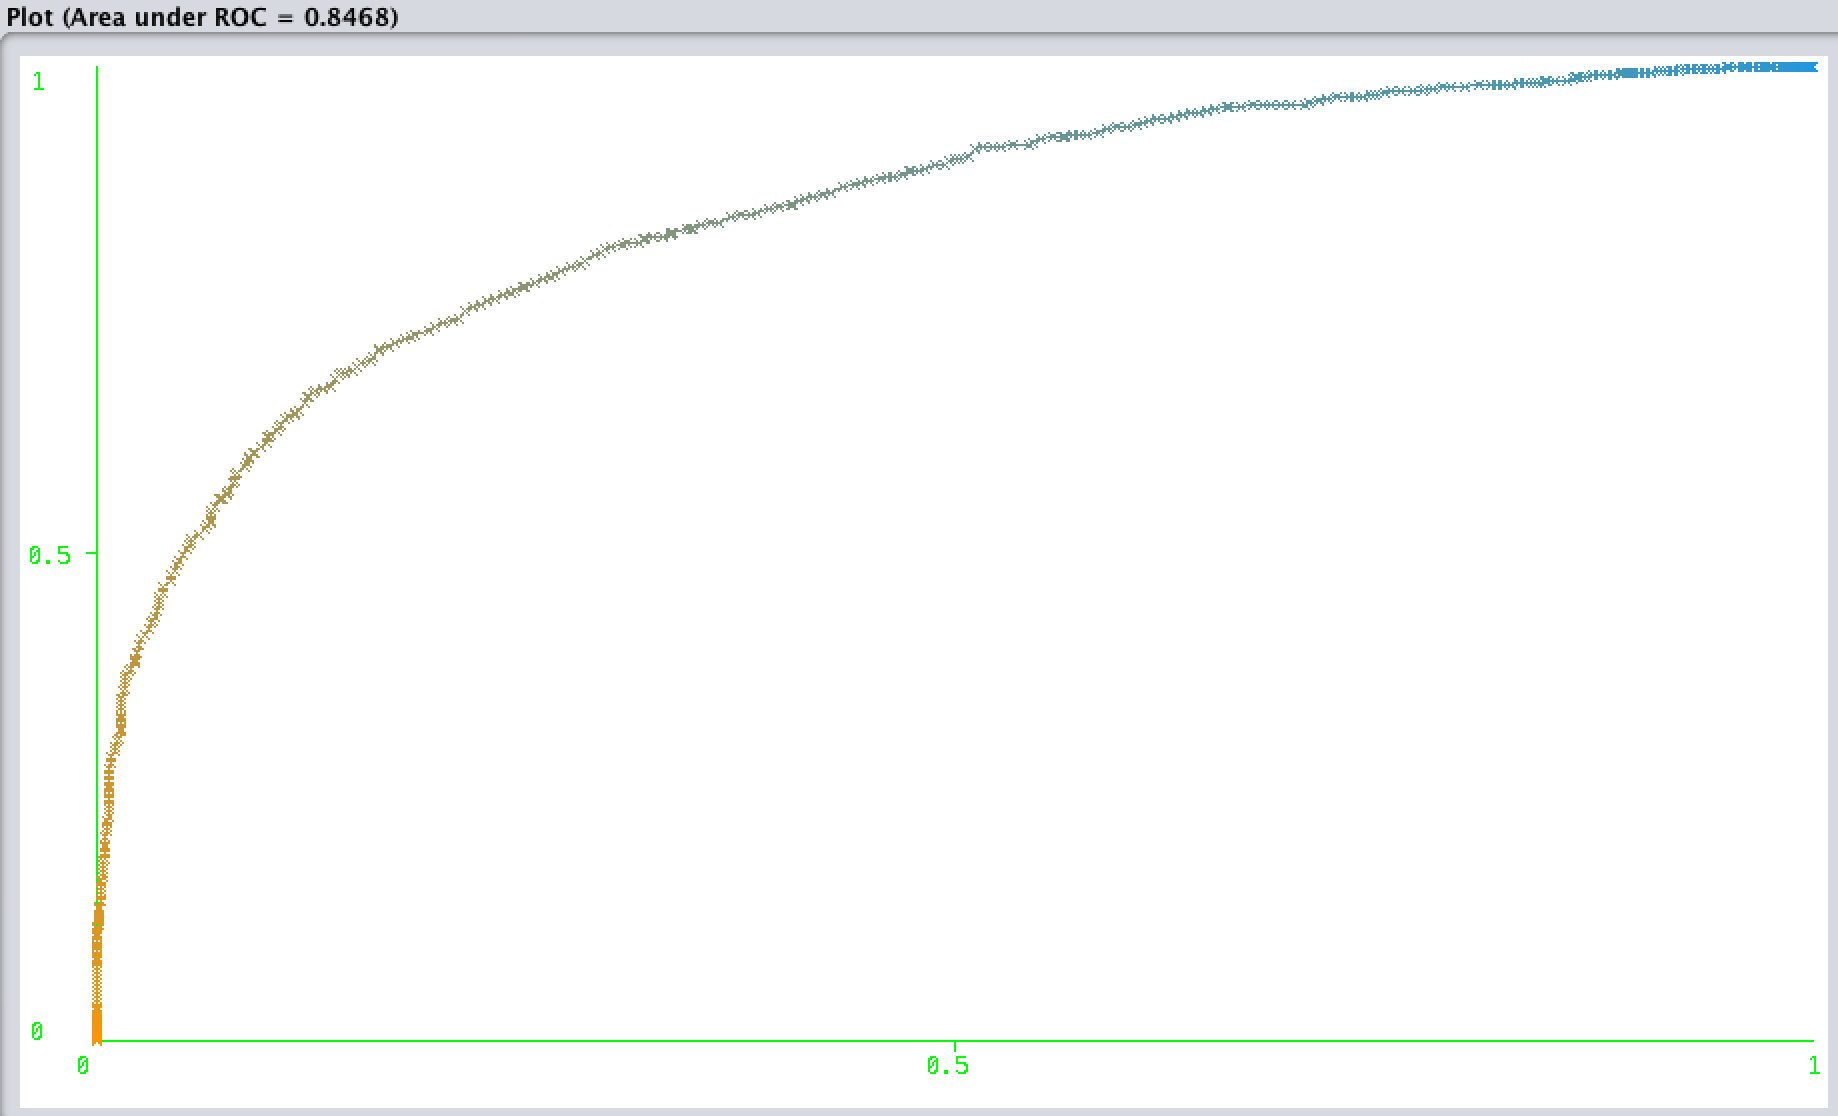
\includegraphics[width=1.0\textwidth]{img/rocResult.png}
	\caption{ROC curve for Cost-Sensitive Random Forest}
	\label{fig:rocCurve}
\end{figure}

% TODO: Add test set description here

Analyzing the results of the prediction framework led to following technical findings. Firstly, decision trees as base classifier and especially the ensemble algorithm Random Forest outperformed the Support Vector machines. Thus it can be followed that a rule-based classification approach suits the prediction of Customer Satisfaction based on usage features better than a functional approach like SVM. Regarding preprocessing and transformation of the data set, oversampling drastically improved the performance of the classifier. This shifted attention of the author to an intensive research and experimenting phase to tackle the class imbalance problem whereby the SMOTE algorithm finally turned out to be well suited since it could keep the performance in training high but did not overfit the trained model too much. Quite some effort was put on finding a preferred method to handle missing data. Although in the literature, mean and mode imputation were sometimes criticized to introduce bias in the data and thus diminish power of classification, the prediction framework selected the rather simple but broadly used method when achieving the best results. This was a bit surprising to the author as the k-nearest-neighbor implementation was considered as more sophisticated and also yielded better results in dedicated research experiments as outlined for instance in \cite{batista2003analysis}.

The following chapter will conclude the thesis by taking again a look on the results to draw consequences out of them. 